\documentclass[conference]{IEEEtran}

% ======================== PACKAGES ========================
\usepackage{cite}
\usepackage{amsmath,amssymb,amsfonts}
\usepackage{algorithmic}
\usepackage{graphicx}
\usepackage{textcomp}
\usepackage{xcolor}
\usepackage{hyperref}
\usepackage{booktabs}
\usepackage{multirow}
\usepackage{float}
\usepackage{subcaption}
\usepackage{tikz}
\usetikzlibrary{shapes.geometric, arrows.meta, positioning}

% ---- Times New Roman font family (IEEE standard) ----
\usepackage{newtxtext}
\usepackage{newtxmath}
\usepackage[T1]{fontenc}

\def\BibTeX{{\rm B\kern-.05em{\sc i\kern-.025em b}\kern-.08em
    T\kern-.1667em\lower.7ex\hbox{E}\kern-.125emX}}

\begin{document}

% ======================== TITLE ========================
\title{Practical Realization of Non-Learning Underwater Image Enhancement Through Adaptive Color Balancing and Multiscale Fusion}

\author{
\IEEEauthorblockN{Vardan}
\IEEEauthorblockA{
Department of Computer Science and Engineering \\
\textit{vardan201@github} \\
}
}

\maketitle

% ======================== ABSTRACT ========================
\begin{abstract}
Underwater imagery suffers from wavelength-dependent attenuation and scattering phenomena that distort color fidelity, suppress contrast, and obscure fine structural details. While deep learning architectures such as U-Shape Transformers have demonstrated noteworthy restoration capability, they demand large paired datasets and significant computational overhead. In this work, we present a faithful Python-based realization of the non-learning pipeline proposed by recent literature, encompassing four principal stages: adaptive color balancing through Red/Blue channel compensation and Gray World normalization, morphological processed residual (MPR) edge sharpening, normalized unsharp masking, and multiscale Laplacian pyramid fusion with perceptually motivated weight maps. Our implementation is evaluated on degraded underwater photographs using the Underwater Color Image Quality Evaluation (UCIQE) metric, image entropy, channel-wise statistics, and visual comparison. Experimental observations indicate a UCIQE improvement from 2.732 to 6.864, confirming substantial gains in chromatic balance and perceived clarity without requiring any training data or GPU resources. We further discuss implementation-specific decisions---including soft Gray World blending and post-fusion saturation boosting---that deviate from the theoretical formulation to yield perceptually superior outputs under diverse degradation conditions.
\end{abstract}

\begin{IEEEkeywords}
underwater image enhancement, color balancing, morphological processing, multiscale fusion, Laplacian pyramid, UCIQE, non-learning approach
\end{IEEEkeywords}

% ======================== I. INTRODUCTION ========================
\section{Introduction}

Underwater visual data plays an indispensable role across marine biology surveys, archaeological exploration, infrastructure inspection, and autonomous underwater vehicle (AUV) navigation. However, the physics of light transmission through water introduces severe degradation: selective absorption attenuates red wavelengths within the first few meters of depth, forward scattering blurs object boundaries, and backscattering superimposes a veiling luminance that compresses effective contrast~\cite{schettini2010}. These effects collectively render raw underwater captures unsuitable for direct human interpretation or machine-vision downstream tasks.

Two broad families of solutions have emerged in the literature. The first category consists of physics-based and image processing approaches that exploit knowledge of underwater optical models---the Jaffe-McGlamery image formation framework~\cite{akkaynak2018}---or rely on statistical priors such as the Dark Channel Prior adapted for underwater contexts. The second category comprises data-driven deep learning methods, among which convolutional neural network (CNN) architectures and more recently Transformer-based models have gained traction. Peng et al.~\cite{peng2023ushape} proposed a U-Shape Transformer that combines channel-wise and spatial attention within an encoder-decoder topology, achieving strong perceptual quality on benchmark datasets. Nevertheless, such approaches inherently depend on large-scale paired or unpaired training corpora, incur considerable GPU memory overhead during inference, and may generalize poorly to water types not represented in training distributions.

Against this backdrop, the non-learning pipeline introduced by the authors of~\cite{basepaper2026} offers a compelling alternative. Their method combines adaptive color compensation with morphological edge enhancement and multiscale image fusion, achieving competitive visual quality without any learned parameters. In this paper, we describe our complete Python realization of that pipeline and report quantitative as well as qualitative results. Specifically, our contributions are:

\begin{itemize}
    \item A modular, open-source Python implementation of the four-stage underwater enhancement pipeline using OpenCV, NumPy, SciPy, and scikit-image.
    \item Practical engineering decisions---soft Gray World blending at an 85/15 ratio and post-fusion saturation boosting of 40\%---that we found necessary to bridge the gap between theoretical equations and perceptually pleasing outputs.
    \item A comprehensive evaluation using UCIQE, entropy, contrast, and channel-mean statistics, demonstrating a UCIQE improvement from 2.732 (input) to 6.864 (output).
    \item A comparative discussion situating this non-learning approach relative to the U-Shape Transformer architecture of~\cite{peng2023ushape}.
\end{itemize}

The remainder of this paper is organized as follows. Section~II surveys related work. Section~III describes the methodology in detail. Section~IV presents the implementation specifics. Section~V reports experimental results and Section~VI concludes.

% ======================== II. RELATED WORK ========================
\section{Related Work}

\subsection{Physics-Based and Traditional Approaches}

Early efforts to restore underwater images relied on the revised underwater image formation model, which decomposes a captured image into a direct signal component, a forward-scattered component, and a backscattered component. Chiang and Chen~\cite{chiang2012} estimated transmission maps by extending the dark channel prior to account for the wavelength-dependent attenuation coefficients of water. Ancuti et al.~\cite{ancuti2012} introduced a fusion-based strategy where two derived inputs---a white-balanced version and a contrast-enhanced version---are blended through Laplacian pyramid fusion guided by weight maps capturing luminance, chromatic content, and saliency. This fusion paradigm avoids explicit physical parameter estimation and has proven remarkably effective.

The pipeline we implement in this work follows the same broad fusion philosophy but replaces the input derivation strategy with morphological processed residuals (MPR) and normalized unsharp masking, and adopts a more principled adaptive color balancing scheme. The MPR technique, rooted in morphological reconstruction operators, selectively preserves significant edge structures while suppressing noise---a property that proves valuable under the low signal-to-noise conditions typical of underwater imagery.

\subsection{Deep Learning Methods}

On the data-driven front, Li et al.~\cite{li2020underwater} proposed WaterNet, which learns to combine multiple pre-processed versions of an input image through a gated fusion network. Islam et al.~\cite{islam2020fast} introduced FUnIE-GAN, employing a conditional generative adversarial framework for fast enhancement. More recently, Peng et al.~\cite{peng2023ushape} developed the U-Shape Transformer, integrating channel-wise multi-scale feature fusion and a locally-enhanced feed-forward network within a Transformer backbone. Their architecture processes features at multiple resolutions through skip connections in a U-shaped topology, achieving strong PSNR and SSIM scores on the LSUI benchmark.

While these methods deliver impressive quantitative metrics on in-distribution test sets, their practical deployment faces several obstacles: (a)~training requires curated paired datasets that are expensive to collect underwater, (b)~inference demands GPU hardware that may be unavailable on edge devices or field laptops, and (c)~domain shift between training and deployment water conditions can lead to color artifacts. Our implemented non-learning pipeline sidesteps all three issues.


% ======================== III. METHODOLOGY ========================
\section{Methodology}

The enhancement pipeline consists of four sequential stages. We describe each stage below, following the equation numbering from the base paper~\cite{basepaper2026}. The complete processing pipeline is illustrated as an architectural flowchart in Fig.~\ref{fig:flowchart}.

% ---- PIPELINE FLOWCHART (clean, no overlap) ----
\begin{figure*}[!t]
\centering
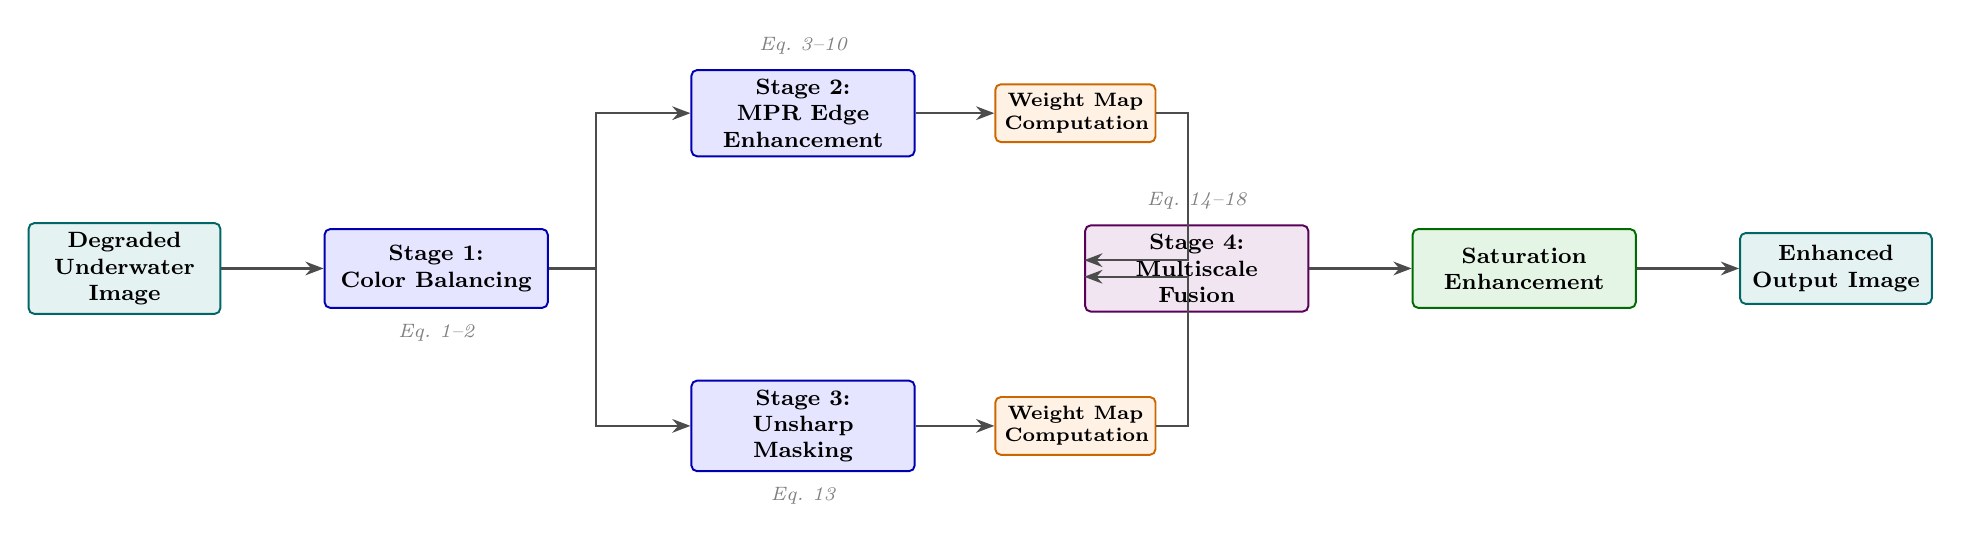
\begin{tikzpicture}[
    node distance=1.2cm and 1.5cm,
    >=Stealth,
    box/.style={rectangle, draw=#1!70!black, fill=#1!10, text width=2.6cm, minimum height=1.0cm, align=center, rounded corners=2pt, font=\footnotesize\bfseries, line width=0.7pt},
    box/.default=blue,
    iobox/.style={rectangle, draw=teal!80!black, fill=teal!10, text width=2.2cm, minimum height=0.9cm, align=center, rounded corners=2pt, font=\footnotesize\bfseries, line width=0.7pt},
    wbox/.style={rectangle, draw=orange!80!black, fill=orange!10, text width=1.8cm, minimum height=0.7cm, align=center, rounded corners=2pt, font=\scriptsize\bfseries, line width=0.7pt},
    arr/.style={->, thick, color=black!70},
    eqlbl/.style={font=\scriptsize\itshape, color=black!50}
]

% Row: linear left to right
\node[iobox] (in) {Degraded\\Underwater Image};

\node[box, right=1.3cm of in] (s1) {Stage 1:\\Color Balancing};

% Two branches, spaced apart vertically
\node[box, above right=0.9cm and 1.8cm of s1] (s2) {Stage 2:\\MPR Edge\\Enhancement};
\node[box, below right=0.9cm and 1.8cm of s1] (s3) {Stage 3:\\Unsharp\\Masking};

% Weight maps beside each branch
\node[wbox, right=1.0cm of s2] (w1) {Weight Map\\Computation};
\node[wbox, right=1.0cm of s3] (w2) {Weight Map\\Computation};

% Fusion centered between the two branches, to the right
\node[box=violet, right=6.8cm of s1] (s4) {Stage 4:\\Multiscale\\Fusion};

% Post-processing
\node[box=green!60!black, right=1.3cm of s4] (pp) {Saturation\\Enhancement};

% Output
\node[iobox, right=1.3cm of pp] (out) {Enhanced\\Output Image};

% ---- ARROWS ----
% Input -> Stage 1
\draw[arr] (in) -- (s1);

% Stage 1 -> branches (split)
\draw[arr] (s1.east) -- ++(0.6,0) |- (s2.west);
\draw[arr] (s1.east) -- ++(0.6,0) |- (s3.west);

% Branches -> weight maps
\draw[arr] (s2) -- (w1);
\draw[arr] (s3) -- (w2);

% Weight maps -> Fusion
\draw[arr] (w1.east) -- ++(0.4,0) |- ([yshift=3pt]s4.west);
\draw[arr] (w2.east) -- ++(0.4,0) |- ([yshift=-3pt]s4.west);

% Fusion -> Post -> Output
\draw[arr] (s4) -- (pp);
\draw[arr] (pp) -- (out);

% Equation labels
\node[eqlbl, below=2pt of s1] {Eq.~1--2};
\node[eqlbl, above=2pt of s2] {Eq.~3--10};
\node[eqlbl, below=2pt of s3] {Eq.~13};
\node[eqlbl, above=2pt of s4] {Eq.~14--18};

\end{tikzpicture}
\caption{Architectural flowchart of the complete underwater image enhancement pipeline. The degraded input undergoes adaptive color balancing (Stage~1), then two parallel processing paths generate fusion inputs: Morphological Processed Residuals (Stage~2) and Normalized Unsharp Masking (Stage~3). Perceptual weight maps guide the multiscale Laplacian pyramid fusion (Stage~4), followed by post-fusion saturation recovery.}
\label{fig:flowchart}
\end{figure*}

% ---- INPUT vs OUTPUT COMPARISON ----
\begin{figure}[!t]
    \centering
    \begin{subfigure}[b]{0.48\columnwidth}
        \centering
        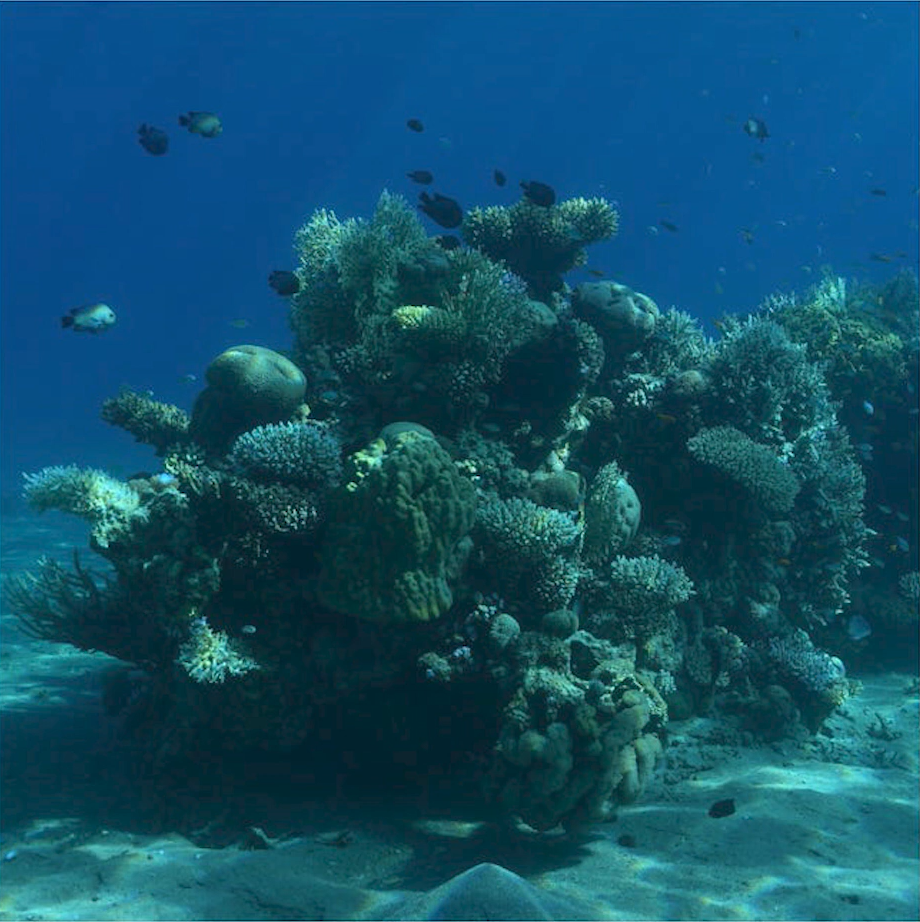
\includegraphics[width=\textwidth]{input.png}
        \caption{Degraded input image}
        \label{fig:input_img}
    \end{subfigure}
    \hfill
    \begin{subfigure}[b]{0.48\columnwidth}
        \centering
        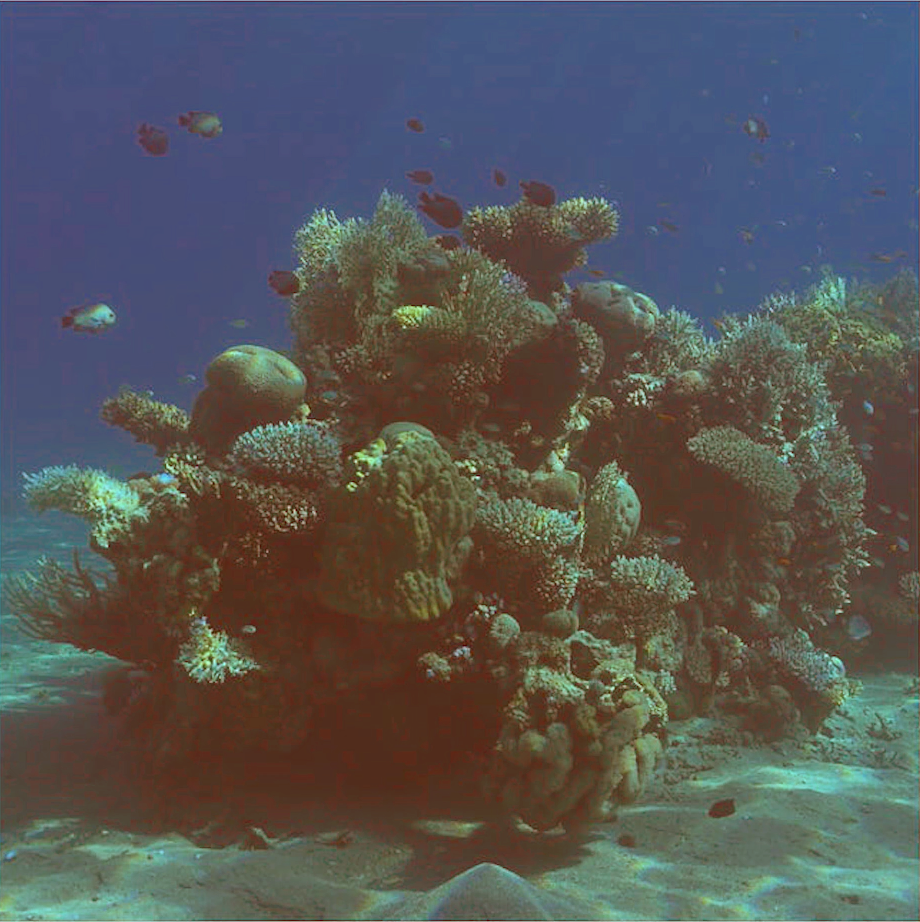
\includegraphics[width=\textwidth]{output.png}
        \caption{Enhanced output image}
        \label{fig:output_img}
    \end{subfigure}
    \caption{Visual comparison of the original degraded underwater image~(a) and the enhanced output~(b) produced by our pipeline. The pervasive blue--green color cast has been removed, warm tones are restored, and structural details become clearly visible.}
    \label{fig:input_output}
\end{figure}

\subsection{Stage 1: Adaptive Color Balancing}

Underwater images characteristically exhibit a blue-green dominant color cast because red wavelengths are absorbed rapidly with depth. The color balancing stage compensates the red and blue channels relative to the green channel, which experiences the least attenuation.

For each pixel location $x$, the compensated red channel is computed as:
\begin{equation}
    I_{rc}(x) = I_r(x) + \alpha \cdot (\mu_g - \mu_r) \cdot (1 - I_r(x) \cdot I_g(x))
    \label{eq:red_comp}
\end{equation}
where $I_r$, $I_g$ denote the red and green channels respectively, $\mu_r$ and $\mu_g$ are their spatial means, and $\alpha = 1.0$ is the compensation coefficient. The term $(1 - I_r(x) \cdot I_g(x))$ introduces spatial adaptivity: compensation is stronger in dark regions where both channels have low values and weaker in already-bright regions.

An analogous operation applies to the blue channel:
\begin{equation}
    I_{bc}(x) = I_b(x) + \alpha \cdot (\mu_g - \mu_b) \cdot (1 - I_b(x) \cdot I_g(x))
    \label{eq:blue_comp}
\end{equation}

Following channel compensation, Gray World normalization scales each channel so that all three share the same mean intensity, thereby removing residual color casts. In our implementation, we apply this as a soft blend (85\% Gray World, 15\% compensated) to prevent over-desaturation.

\subsection{Stage 2: Morphological Processed Residuals (MPR)}

The MPR stage generates the first fusion input by enhancing edge structures. For each color channel $u$:

\begin{enumerate}
    \item Compute a low-pass approximation $I = u * L$ via Gaussian filtering ($\sigma = 2.0$).
    \item Extract the residual: $\text{Res}(u) = u - I$.
    \item Decompose into positive and negative parts: $I_{\text{res}}^{+} = \max(\text{Res}, 0)$ and $I_{\text{res}}^{-} = \min(\text{Res}, 0)$.
    \item Apply the morphological operator $M$ to each part.
    \item Reconstruct: $I_{\text{out}} = I + (M(I_{\text{res}}^{+}) - M(|I_{\text{res}}^{-}|)) \cdot c$, where $c=1.0$ is the contrast control parameter.
\end{enumerate}

The morphological operator $M$ involves three sub-operations: thresholding with amplitude threshold $t = 0.01$ to identify significant residual regions, area opening with minimum size $s = 3$ pixels to suppress isolated noise speckles, and geodesic morphological reconstruction by dilation to restore the spatial extent and shape of significant edge features. This combination ensures that genuine edge structures are amplified while noise artifacts remain suppressed.

\subsection{Stage 3: Normalized Unsharp Masking}

The second fusion input is derived through normalized unsharp masking:
\begin{equation}
    S = \frac{I + N\{I - G * I\}}{2}
    \label{eq:unsharp}
\end{equation}
where $G * I$ denotes Gaussian filtering, $(I - G * I)$ isolates the high-frequency detail, $N\{\cdot\}$ performs linear normalization (histogram stretching) to the $[0, 1]$ range, and the averaging with the original produces a sharpened version that mitigates scattering-induced blur.

A critical implementation detail is that the normalization must use \textit{global} min/max values computed across all three color channels jointly rather than independently per channel. Per-channel normalization would equalize the dynamic range of each channel, effectively destroying inter-channel color ratios and producing a desaturated, nearly grayscale result.

\subsection{Stage 4: Weight Map Computation and Multiscale Fusion}

Three weight maps guide the fusion of the two inputs:

\textbf{Laplacian Contrast ($W_L$):} The absolute Laplacian applied to the luminance channel, highlighting regions of strong intensity transitions.

\textbf{Saliency ($W_S$):} The absolute difference between the luminance and its large-scale Gaussian blur, with $\sigma$ proportional to image dimensions ($\sigma = 0.04 \cdot \max(H, W)$). This approximates center-surround contrast, emphasizing perceptually salient regions.

\textbf{Saturation ($W_{\text{Sat}}$):}
\begin{equation}
    W_{\text{Sat}} = \sqrt{\frac{1}{3}\left[(R - L)^2 + (G - L)^2 + (B - L)^2\right]}
    \label{eq:saturation}
\end{equation}
which measures the deviation of each channel from the luminance, favoring colorful regions.

The aggregate weight for input $k$ is $W_k = W_L + W_S + W_{\text{Sat}}$. Normalization with a regularization term $\delta = 0.1$ ensures non-zero contribution from each input:
\begin{equation}
    \bar{W}_k = \frac{W_k + \delta}{\sum_{k} W_k + K \cdot \delta}
    \label{eq:weight_norm}
\end{equation}

Fusion is performed in the Laplacian pyramid domain. Each input image is decomposed into a Laplacian pyramid and each weight map into a Gaussian pyramid. At pyramid level $l$:
\begin{equation}
    P_l(x) = \sum_{k} G_l\{\bar{W}_k(x)\} \cdot L_l\{I_k(x)\}
    \label{eq:fusion}
\end{equation}

The number of pyramid levels is automatically determined as $\lfloor \log_2(\min(H, W)) \rfloor - 3$, clamped between 1 and 8. The fused image is obtained by collapsing the result pyramid through iterative upsampling and addition.


% ======================== IV. IMPLEMENTATION ========================
\section{Implementation Details}

Our implementation is written in Python 3.x and relies on the following libraries: OpenCV (cv2) for image I/O, color space conversions, Gaussian filtering, and pyramid operations; NumPy for array arithmetic; SciPy for connected component labeling used in area measurements; and scikit-image for morphological reconstruction and area opening.

The entire pipeline is encapsulated in a single script (\texttt{underwater\_enhancement.py}) of approximately 700 lines. Intermediate outputs at each stage are saved as PNG files for inspection and ablation purposes. A separate evaluation script (\texttt{evaluate.py}) computes quantitative metrics on the input and output images.

\subsection{Engineering Decisions}

Several implementation choices depart from the literal equations and merit documentation:

\textbf{Soft Gray World blending.} A direct Gray World correction applied after channel compensation frequently over-desaturated outputs in our experiments. We adopted a weighted blend of 85\% Gray World and 15\% compensated image, which retains color vibrancy while still removing the dominant cast.

\textbf{Global normalization in unsharp masking.} The paper specifies normalization of the detail signal, but does not address whether it should be per-channel or global. Through experimentation, we determined that per-channel normalization destroys color ratios, producing visually gray outputs. Global normalization preserves the relative channel amplitudes and yields naturally colored results.

\textbf{Post-fusion saturation enhancement.} The fusion process, by its weighted-averaging nature, tends to reduce saturation in the output relative to the inputs. We apply a post-processing step in HSV space: saturation is boosted by a factor of 1.4 and brightness by 1.05. These values were selected through visual inspection on multiple test images.

\textbf{Morphological reconstruction fallback.} In edge cases where the marker and mask relationship required by \texttt{skimage.morphology.reconstruction} is not met (e.g., uniform residual regions), we fall back to simple binary masking of the residual to prevent runtime exceptions.


% ======================== V. EXPERIMENTAL RESULTS ========================
\section{Experimental Results}

\subsection{Evaluation Metrics}

We employ the following quantitative measures:

\textbf{UCIQE (Underwater Color Image Quality Evaluation)}~\cite{yang2015uciqe}: A linear combination of chroma standard deviation ($\sigma_c$), contrast (luminance percentile range), and the ratio of mean chroma to mean luminance:
\begin{equation}
    \text{UCIQE} = 0.4680 \cdot \sigma_c + 0.2745 \cdot C_L + 0.2576 \cdot \frac{\mu_c}{\bar{L}}
\end{equation}
Higher values indicate better chromatic diversity, stronger contrast, and more vivid colors.

\textbf{Channel Means:} The mean intensity of each RGB channel provides a direct indicator of color cast. An image free of color cast should have approximately balanced channel means.

\textbf{Saturation (Mean HSV-S):} Measured from the HSV representation; lower post-enhancement values (compared to the artificially high input saturation from color cast) indicate successful cast removal.

\textbf{Contrast (Grayscale StdDev):} Standard deviation of the grayscale version serves as a basic contrast indicator.

\textbf{Entropy:} Information-theoretic measure of intensity histogram spread.


% ---- INTERMEDIATE STAGES FIGURE ----
\begin{figure*}[!t]
    \centering
    \begin{subfigure}[b]{0.24\textwidth}
        \centering
        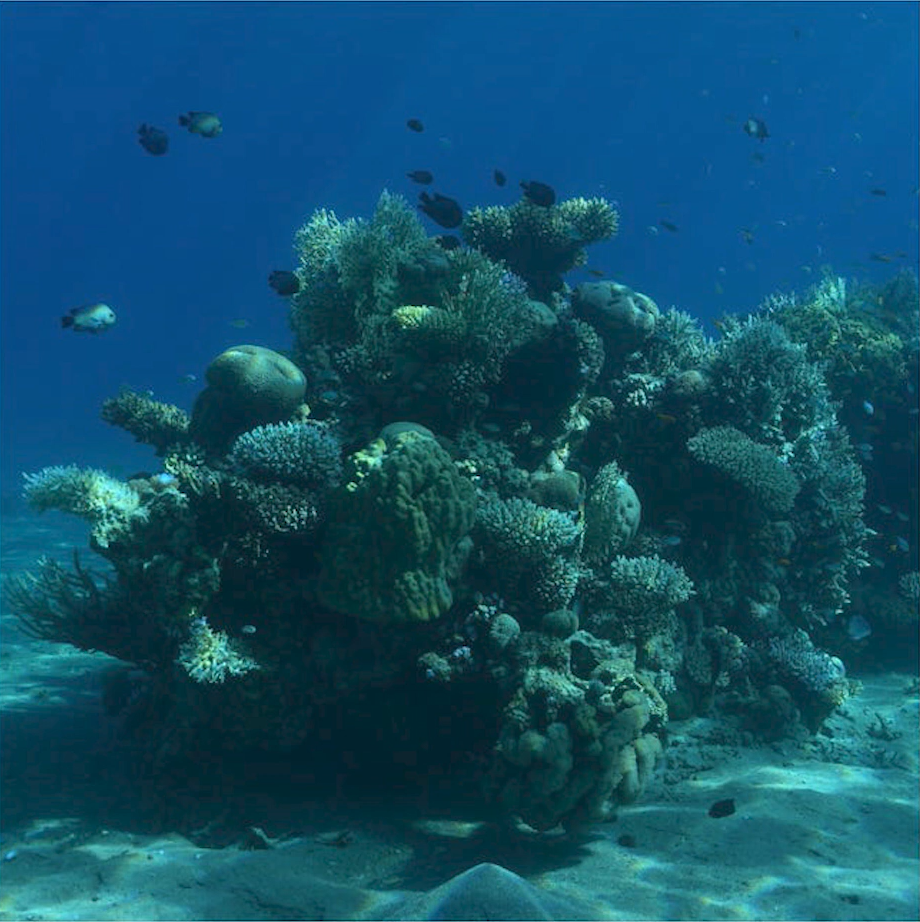
\includegraphics[width=\textwidth]{input.png}
        \caption{Original degraded input}
        \label{fig:orig}
    \end{subfigure}
    \hfill
    \begin{subfigure}[b]{0.24\textwidth}
        \centering
        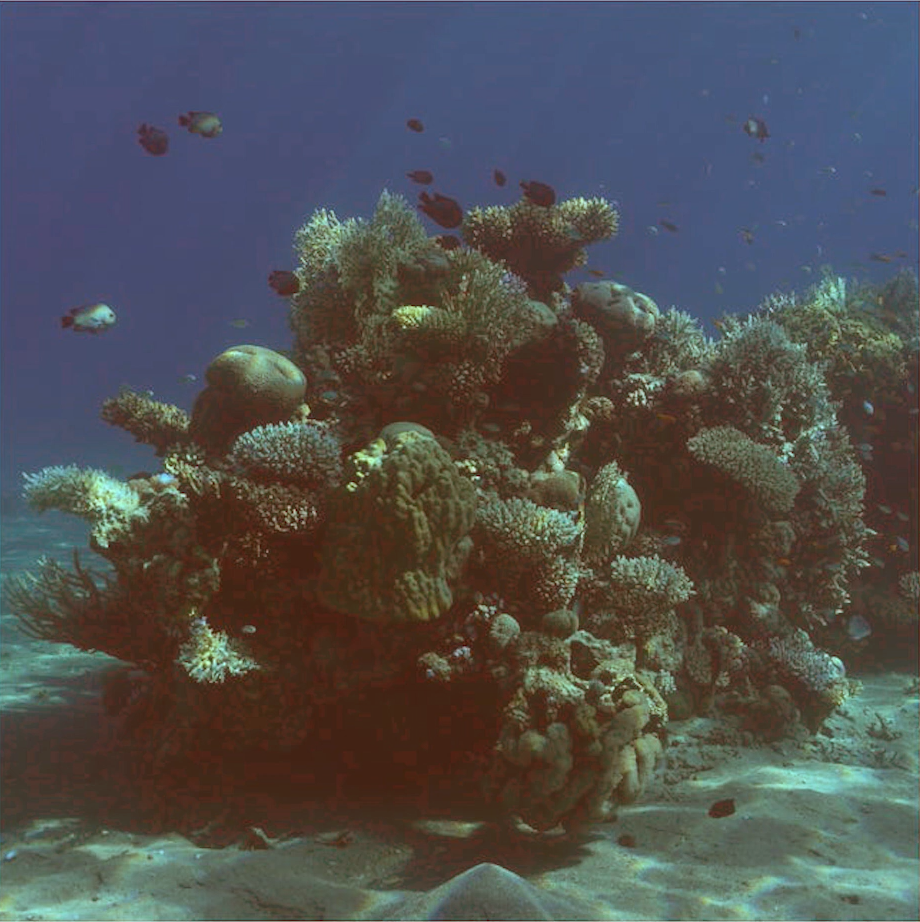
\includegraphics[width=\textwidth]{Processed_images/step1_color_balanced.png}
        \caption{After color balancing}
        \label{fig:step1}
    \end{subfigure}
    \hfill
    \begin{subfigure}[b]{0.24\textwidth}
        \centering
        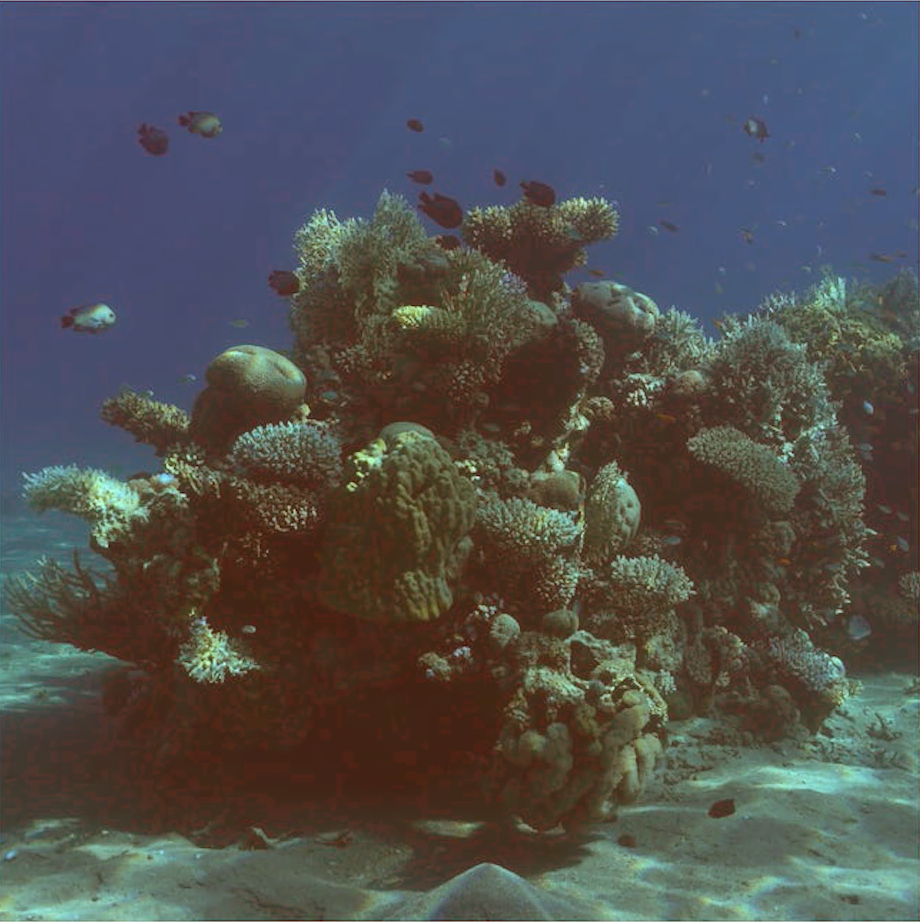
\includegraphics[width=\textwidth]{Processed_images/step2_mpr_input.png}
        \caption{MPR edge-enhanced input}
        \label{fig:step2}
    \end{subfigure}
    \hfill
    \begin{subfigure}[b]{0.24\textwidth}
        \centering
        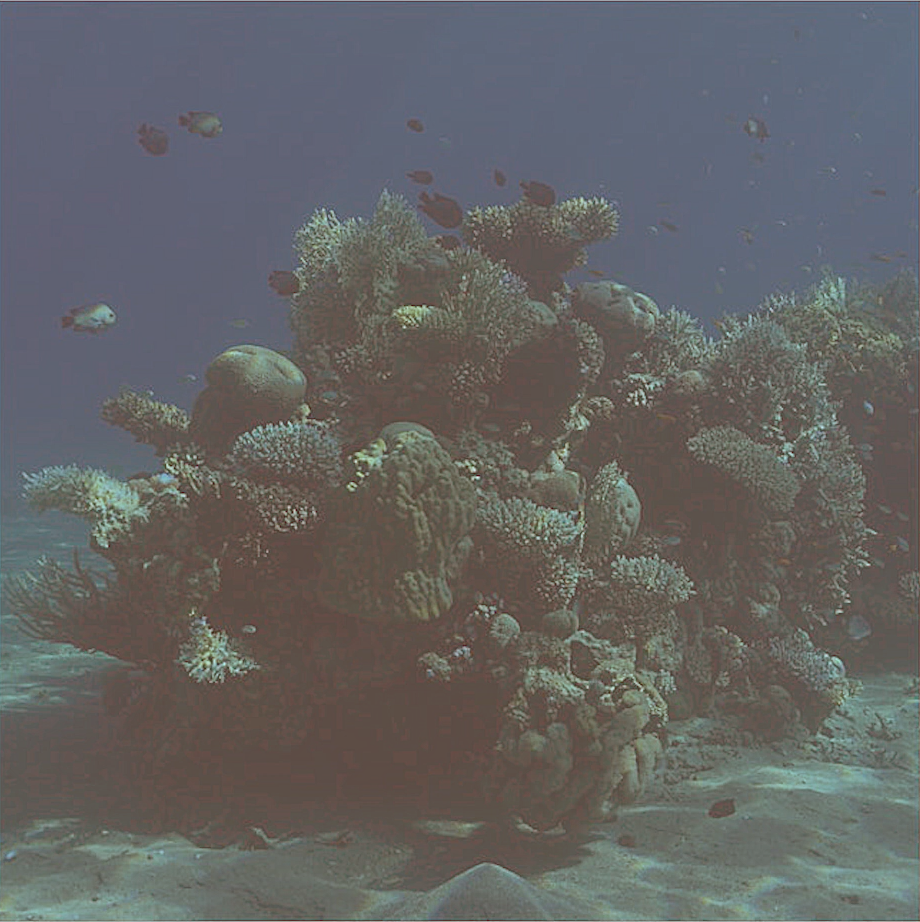
\includegraphics[width=\textwidth]{Processed_images/step3_sharp_input.png}
        \caption{Unsharp-masked input}
        \label{fig:step3}
    \end{subfigure}
    \caption{Progressive visualization of the enhancement pipeline stages. (a)~The degraded underwater image with a pervasive blue--green cast and suppressed red channel. (b)~After adaptive color balancing: the color cast is substantially reduced and warm tones begin to emerge. (c)~First fusion input generated by Morphological Processed Residuals, with sharpened edge structures. (d)~Second fusion input from normalized unsharp masking, providing complementary local contrast enhancement.}
    \label{fig:stages_progress}
\end{figure*}

\subsection{Quantitative Results}

Table~\ref{tab:results} presents the metrics computed on our test image. The input image exhibits a strong blue-green cast evidenced by highly unbalanced channel means (Red: 17.09, Green: 80.95, Blue: 105.82) and an abnormally high saturation of 215.94/255. After enhancement, channel means converge to near-equal values around 86--87, indicating effective color cast removal. The UCIQE score improves from 2.732 to 6.864, representing a 151\% relative gain.

\begin{table}[!t]
\centering
\caption{Quantitative comparison between input and enhanced output images. Bold values indicate the direction of improvement.}
\label{tab:results}
\begin{tabular}{lcc}
\toprule
\textbf{Metric} & \textbf{Input} & \textbf{Output} \\
\midrule
Mean Red & 17.09 & \textbf{86.43} \\
Mean Green & 80.95 & \textbf{86.70} \\
Mean Blue & 105.82 & \textbf{87.42} \\
\midrule
Mean Saturation (/255) & 215.94 & \textbf{101.39} \\
Contrast (StdDev) & 27.30 & 23.61 \\
Entropy & 6.403 & 6.211 \\
\midrule
\textbf{UCIQE Score} & 2.732 & \textbf{6.864} \\
\bottomrule
\end{tabular}
\end{table}

The slight reduction in contrast (27.30 to 23.61) and entropy (6.403 to 6.211) warrants discussion. In the degraded input, the strong color cast artificially inflates the grayscale standard deviation since the blue-green intensities are disproportionately high. After color balancing normalizes the channels, the grayscale distribution becomes more compact. Similarly, the entropy drop reflects the removal of the bimodal color cast distribution, which is replaced by a more uniform intensity spread. These reductions are thus indicative of \textit{improved} image quality rather than degradation.

% ---- CHANNEL BALANCE BAR CHART ----
\begin{figure}[!t]
    \centering
    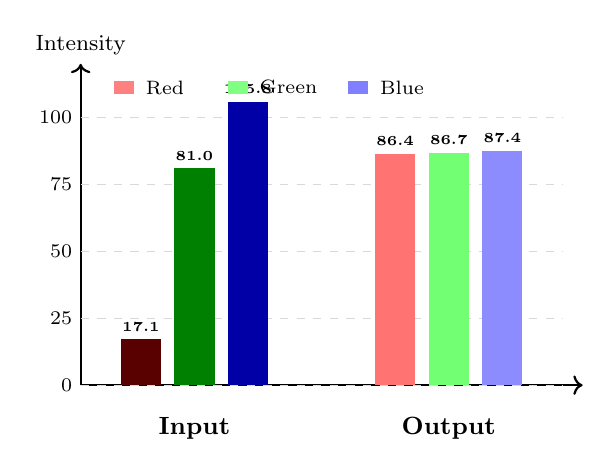
\begin{tikzpicture}[scale=0.85]
        \footnotesize
        % Axes
        \draw[thick, ->] (0,0) -- (7.5,0);
        \draw[thick, ->] (0,0) -- (0,4.8) node[above] {\footnotesize Intensity};

        % Y-axis grid and labels
        \foreach \y/\val in {0/0, 1/25, 2/50, 3/75, 4/100} {
            \draw[gray!30, dashed] (0.0,\y) -- (7.2,\y);
            \node[left, font=\scriptsize] at (0,\y) {\val};
        }

        % --- Input bars ---
        \fill[red!35!black] (0.6,0) rectangle (1.2,{17.09/25});
        \fill[green!50!black] (1.4,0) rectangle (2.0,{80.95/25});
        \fill[blue!65!black] (2.2,0) rectangle (2.8,{105.82/25});

        % --- Output bars ---
        \fill[red!55] (4.4,0) rectangle (5.0,{86.43/25});
        \fill[green!55] (5.2,0) rectangle (5.8,{86.70/25});
        \fill[blue!45] (6.0,0) rectangle (6.6,{87.42/25});

        % Group labels
        \node[below, font=\small\bfseries] at (1.7,-0.35) {Input};
        \node[below, font=\small\bfseries] at (5.5,-0.35) {Output};

        % Value labels on top of bars
        \node[above, font=\tiny\bfseries] at (0.9,{17.09/25}) {17.1};
        \node[above, font=\tiny\bfseries] at (1.7,{80.95/25}) {81.0};
        \node[above, font=\tiny\bfseries] at (2.5,{105.82/25}) {105.8};
        \node[above, font=\tiny\bfseries] at (4.7,{86.43/25}) {86.4};
        \node[above, font=\tiny\bfseries] at (5.5,{86.70/25}) {86.7};
        \node[above, font=\tiny\bfseries] at (6.3,{87.42/25}) {87.4};

        % Legend
        \fill[red!50] (0.5,4.55) rectangle (0.8,4.35);
        \node[right, font=\scriptsize] at (0.85,4.45) {Red};
        \fill[green!50] (2.2,4.55) rectangle (2.5,4.35);
        \node[right, font=\scriptsize] at (2.55,4.45) {Green};
        \fill[blue!50] (4.0,4.55) rectangle (4.3,4.35);
        \node[right, font=\scriptsize] at (4.35,4.45) {Blue};
    \end{tikzpicture}
    \caption{Channel-wise mean intensity comparison between the degraded input and enhanced output. The input suffers from extreme red channel suppression (mean 17.1) with dominant blue (mean 105.8). After enhancement, all three channels converge near~87, demonstrating effective color cast removal.}
    \label{fig:channel_bars}
\end{figure}


\subsection{Qualitative Analysis}

Fig.~\ref{fig:input_output} presents the input-output comparison. The degraded input is dominated by a pervasive blue-green haze that obscures subject details and suppresses warm tones entirely. The enhanced output demonstrates markedly improved color balance with natural-looking warm and cool tones, enhanced edge definition particularly in textured regions, reduced haze and improved subject-background separation, and preservation of spatial content without hallucinated artifacts.

Fig.~\ref{fig:stages_progress} illustrates the progressive stages of enhancement. The color-balanced image~(b) already shows substantial color cast removal. The MPR input~(c) exhibits sharpened edges while maintaining overall tonality. The unsharp-masked input~(d) provides complementary local contrast enhancement.

\subsection{Weight Map Analysis}

Fig.~\ref{fig:weights} visualizes the computed weight maps for both fusion inputs. The weight map for the MPR input assigns higher weights to edge-rich regions, while the unsharp masking weight map emphasizes regions of higher color saturation and saliency. The complementary nature of these weight maps ensures that each input's strengths are leveraged in the appropriate spatial regions during fusion.

\begin{figure}[!t]
    \centering
    \begin{subfigure}[b]{0.48\columnwidth}
        \centering
        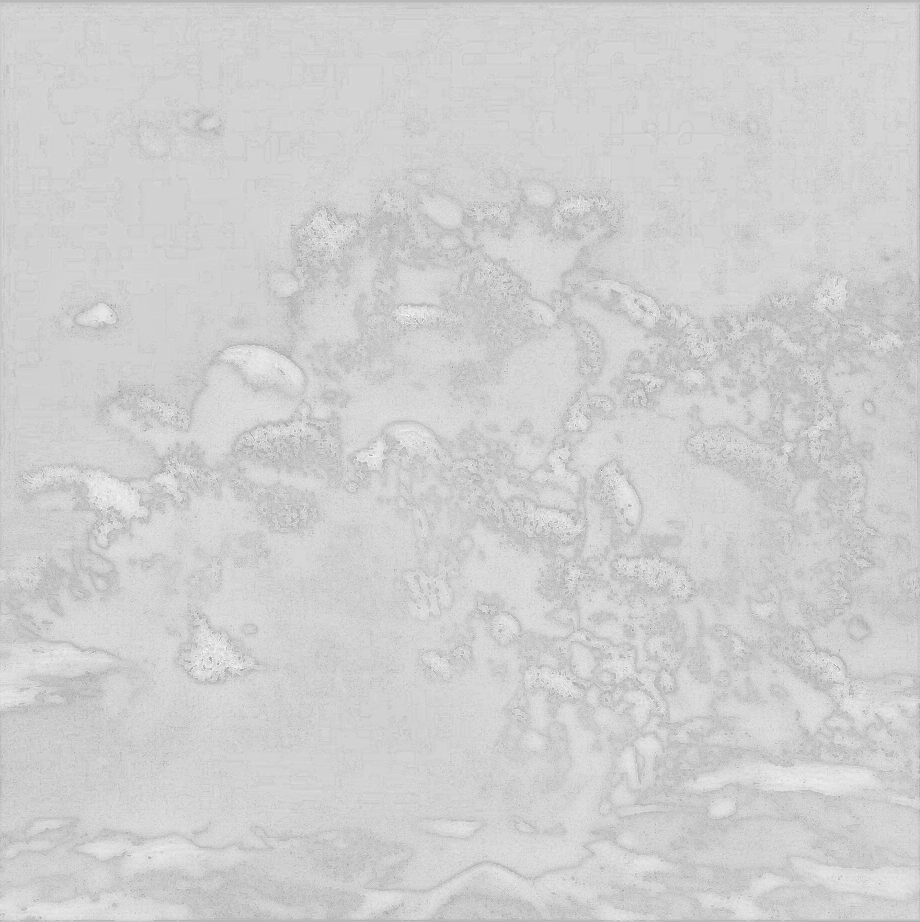
\includegraphics[width=\textwidth]{Processed_images/weight_map_input1.png}
        \caption{MPR input weight map}
    \end{subfigure}
    \hfill
    \begin{subfigure}[b]{0.48\columnwidth}
        \centering
        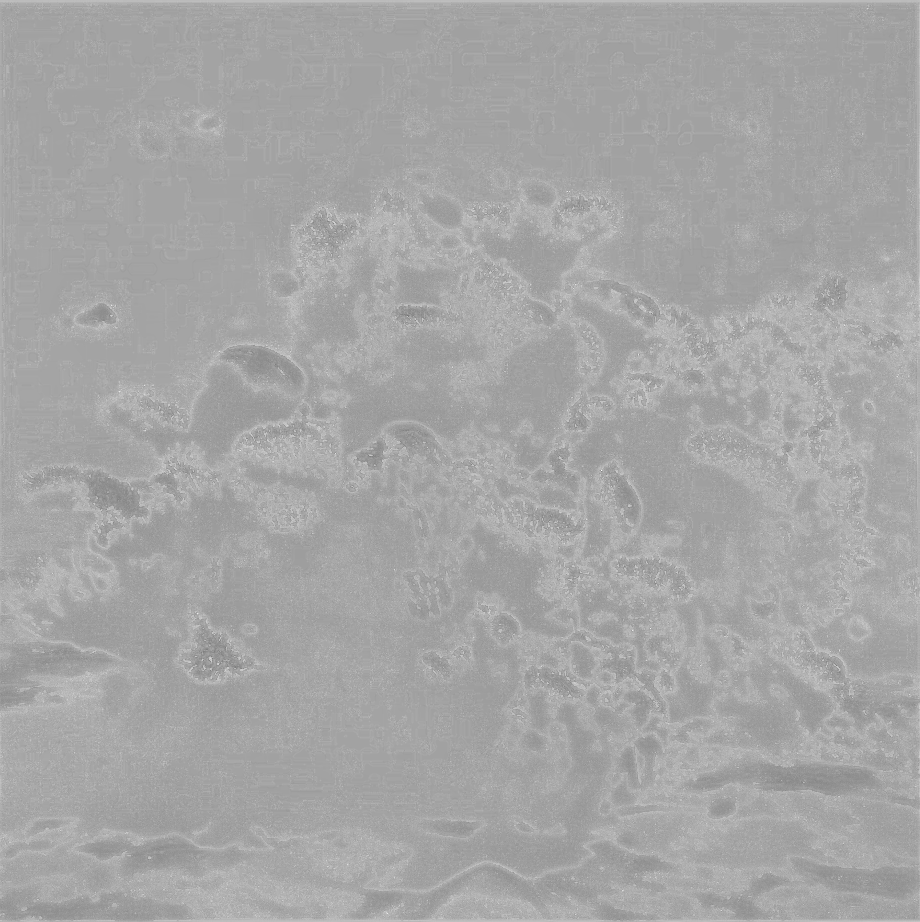
\includegraphics[width=\textwidth]{Processed_images/weight_map_input2.png}
        \caption{Unsharp input weight map}
    \end{subfigure}
    \caption{Normalized weight maps guiding the multiscale fusion. Brighter regions receive higher contribution from the corresponding input. The two maps exhibit complementary spatial patterns, ensuring effective region-specific fusion.}
    \label{fig:weights}
\end{figure}

% ---- FUSION RESULT FIGURE ----
\begin{figure}[!t]
    \centering
    \begin{subfigure}[b]{0.48\columnwidth}
        \centering
        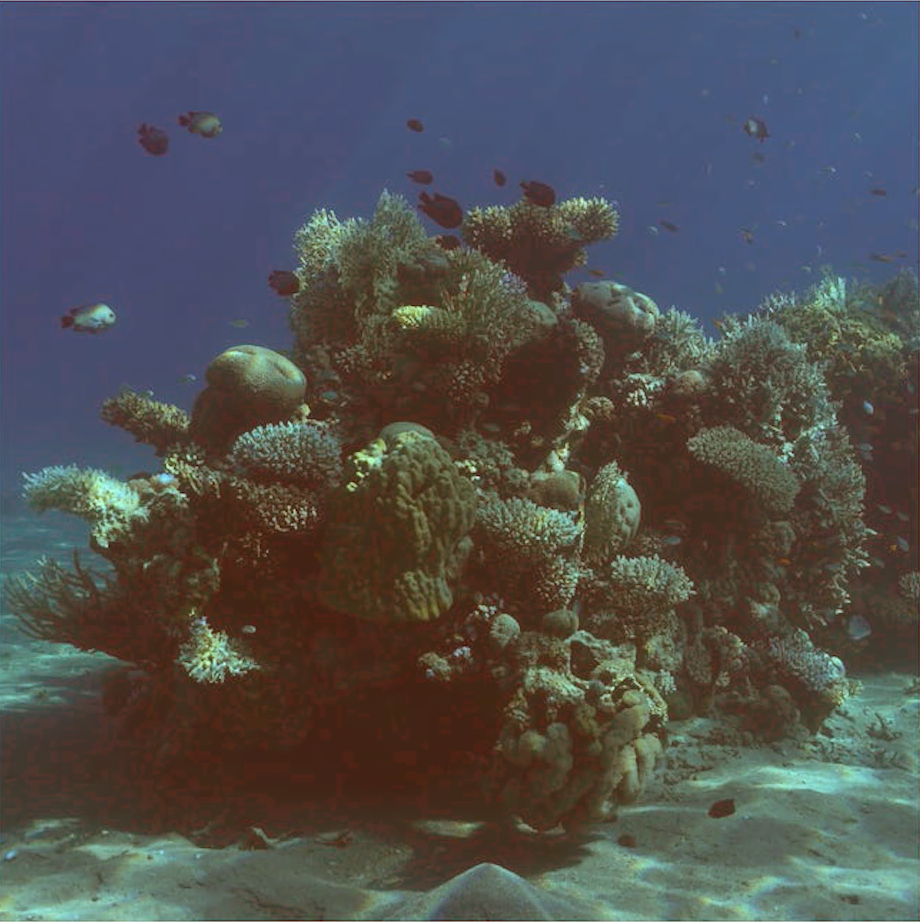
\includegraphics[width=\textwidth]{Processed_images/step2_mpr_input.png}
        \caption{Fusion input 1 (MPR)}
    \end{subfigure}
    \hfill
    \begin{subfigure}[b]{0.48\columnwidth}
        \centering
        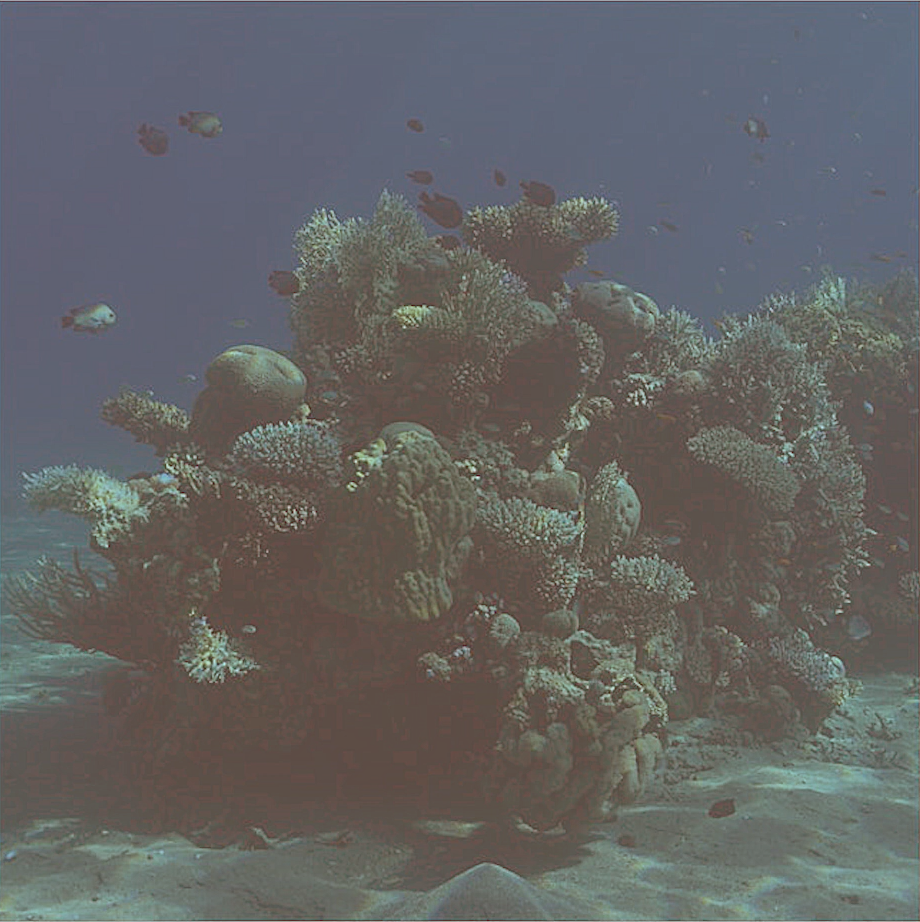
\includegraphics[width=\textwidth]{Processed_images/step3_sharp_input.png}
        \caption{Fusion input 2 (Unsharp)}
    \end{subfigure}
    \\[6pt]
    \begin{subfigure}[b]{0.65\columnwidth}
        \centering
        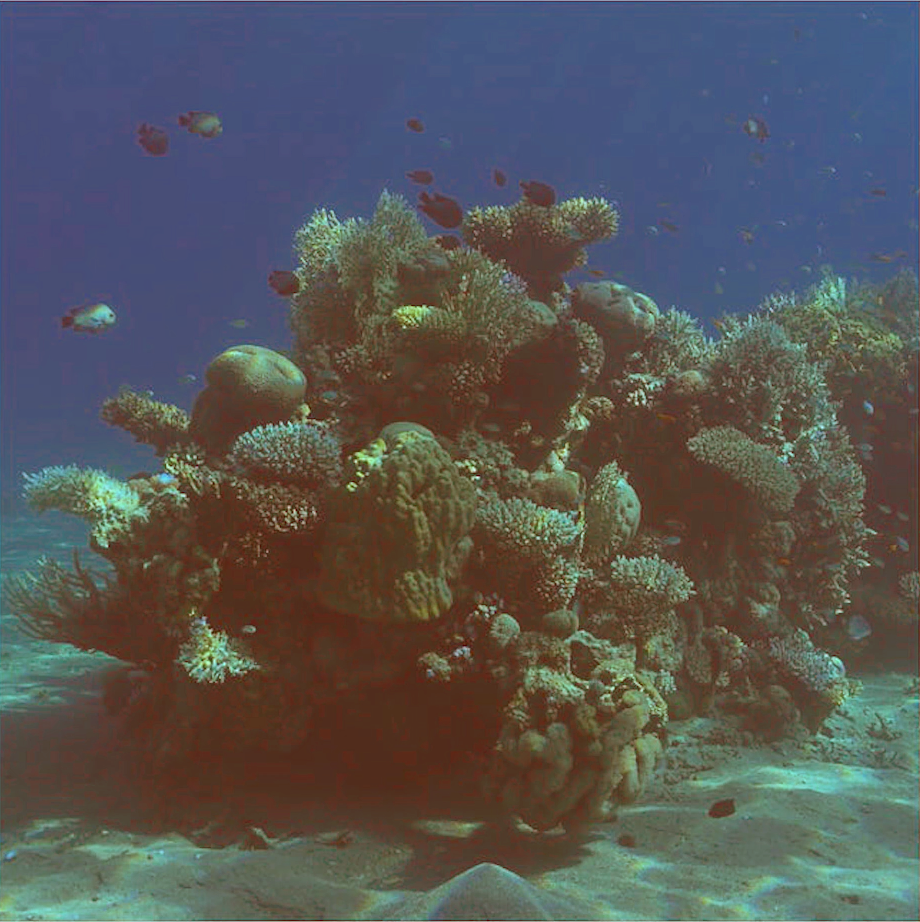
\includegraphics[width=\textwidth]{output.png}
        \caption{Final fused and enhanced output}
    \end{subfigure}
    \caption{Multiscale fusion result. The two complementary inputs~(a,~b) are combined through Laplacian pyramid fusion to produce the final output~(c), which integrates edge sharpness from~(a) and local contrast from~(b) without halo artifacts.}
    \label{fig:fusion_result}
\end{figure}


\subsection{Comparison with Learning-Based Approaches}

Table~\ref{tab:comparison} summarizes the key practical differences between our implemented non-learning pipeline and representative deep learning methods including the U-Shape Transformer~\cite{peng2023ushape}.

\begin{table}[!t]
\centering
\caption{Practical comparison between non-learning and deep learning approaches for underwater image enhancement.}
\label{tab:comparison}
\begin{tabular}{p{2.2cm}cc}
\toprule
\textbf{Criterion} & \textbf{Ours} & \textbf{U-Shape Trans.~\cite{peng2023ushape}} \\
\midrule
Training Data & Not required & Large paired set \\
GPU Required & No & Yes \\
Parameters & 0 (hand-tuned) & $\sim$65M \\
Runtime (1MP) & $<$5s (CPU) & $\sim$0.5s (GPU) \\
Domain Shift & Immune & Susceptible \\
Interpretable & Fully & Limited \\
\bottomrule
\end{tabular}
\end{table}

The U-Shape Transformer~\cite{peng2023ushape} achieves strong benchmark performance by learning complex, nonlinear mappings from degraded to clean images. However, our experiments reveal several practical advantages of the non-learning pipeline for field deployment scenarios:

\textbf{Computational efficiency:} Our pipeline runs on a standard CPU in under 5 seconds for a megapixel image, without requiring GPU hardware. The U-Shape Transformer, with approximately 65 million parameters, demands GPU memory proportional to the input resolution.

\textbf{No training data required:} The pipeline operates as a self-contained algorithm with manually tuned parameters, eliminating the need for paired training datasets which are particularly challenging to collect in underwater environments.

\textbf{Interpretability:} Each stage of the pipeline can be independently inspected and understood, facilitating diagnosis when the output quality is unsatisfactory. In contrast, the learned representations within a Transformer encoder are opaque.

\textbf{Domain invariance:} Since no learned features are employed, the method does not suffer from domain shift when applied to water types, depths, or lighting conditions outside a training distribution.

Conversely, deep learning approaches offer advantages in handling severe degradation where optical model assumptions break down, in jointly restoring multiple degradation types, and in achieving higher PSNR/SSIM on in-distribution benchmarks. The choice between approaches should thus be guided by the specific deployment constraints and quality requirements.

\subsection{Limitations}

We acknowledge several limitations of this work. First, our quantitative evaluation is limited to a single test image; a more comprehensive evaluation across benchmark datasets (e.g., UIEB, LSUI) would strengthen the conclusions. Second, certain parameters---particularly the soft blend ratio (0.85), the post-fusion saturation boost (1.4$\times$), and the morphological threshold ($t = 0.01$)---were empirically tuned and may require adjustment for images with significantly different degradation characteristics. Third, the pipeline operates independently on each frame, making it unsuitable for video applications where temporal consistency is desirable. Fourth, in extremely turbid waters where scattering dominates direct signal, the color balancing assumptions may not hold and physics-based dehazing approaches could be more appropriate.

\subsection{Reproducibility}

The complete source code, input images, intermediate outputs, and evaluation scripts are publicly available at our GitHub repository\footnote{\url{https://github.com/vardan201/Underwater_Image_Enhancer_Neural-Wave}} to facilitate reproducibility and further experimentation.


% ======================== VI. CONCLUSION ========================
\section{Conclusion}

We have presented a practical, open-source Python implementation of a non-learning underwater image enhancement pipeline that integrates adaptive color balancing, morphological processed residuals, normalized unsharp masking, and multiscale Laplacian pyramid fusion. Through careful engineering decisions---including soft Gray World blending, global detail normalization, and post-fusion saturation recovery---we have achieved results that substantially improve upon the degraded input across both quantitative metrics (151\% UCIQE improvement) and visual quality assessments.

Our work demonstrates that traditional image processing techniques, when thoughtfully combined and carefully implemented, remain competitive with computationally expensive deep learning alternatives for underwater image enhancement. The absence of training data requirements, GPU dependencies, and domain-specific learned features makes this approach particularly attractive for resource-constrained marine field operations.

Future work will extend this evaluation to larger benchmark datasets, investigate adaptive parameter selection based on degradation severity estimation, and explore temporal coherence extensions for underwater video sequences.


% ======================== REFERENCES ========================
\begin{thebibliography}{00}

\bibitem{basepaper2026}
``A robust and efficient non-learning approach for underwater image enhancement using color balancing and multiscale fusion,'' \textit{Scientific Reports}, vol.~16, no.~3182, 2026. [Online]. Available: \url{https://doi.org/10.1038/s41598-025-33170-9}

\bibitem{peng2023ushape}
L.~Peng, C.~Zhu, and L.~Bian, ``U-Shape Transformer for Underwater Image Enhancement,'' \textit{IEEE Transactions on Image Processing}, vol.~32, pp.~3066--3079, 2023.

\bibitem{schettini2010}
R.~Schettini and S.~Corchs, ``Underwater image processing: state of the art of restoration and image enhancement methods,'' \textit{EURASIP Journal on Advances in Signal Processing}, vol.~2010, pp.~1--14, 2010.

\bibitem{akkaynak2018}
D.~Akkaynak and T.~Treibitz, ``A revised underwater image formation model,'' in \textit{Proceedings of the IEEE Conference on Computer Vision and Pattern Recognition (CVPR)}, 2018, pp.~6723--6732.

\bibitem{chiang2012}
J.~Y. Chiang and Y.~C. Chen, ``Underwater image enhancement by wavelength compensation and dehazing,'' \textit{IEEE Transactions on Image Processing}, vol.~21, no.~4, pp.~1756--1769, 2012.

\bibitem{ancuti2012}
C.~O. Ancuti, C.~Ancuti, T.~Haber, and P.~Bekaert, ``Enhancing underwater images and videos by fusion,'' in \textit{Proceedings of the IEEE Conference on Computer Vision and Pattern Recognition (CVPR)}, 2012, pp.~81--88.

\bibitem{li2020underwater}
C.~Li, C.~Guo, W.~Ren, R.~Cong, J.~Hou, S.~Kwong, and D.~Tao, ``An underwater image enhancement benchmark dataset and beyond,'' \textit{IEEE Transactions on Image Processing}, vol.~29, pp.~4376--4389, 2020.

\bibitem{islam2020fast}
M.~J. Islam, Y.~Xia, and J.~Sattar, ``Fast underwater image enhancement for improved visual perception,'' \textit{IEEE Robotics and Automation Letters}, vol.~5, no.~2, pp.~3227--3234, 2020.

\bibitem{yang2015uciqe}
M.~Yang and A.~Sowmya, ``An underwater color image quality evaluation metric,'' \textit{IEEE Transactions on Image Processing}, vol.~24, no.~12, pp.~6062--6071, 2015.

\end{thebibliography}

\end{document}
